\subsubsection{Chrysemys --- Painted Turtles}
\begin{center}
\begin{longtabu} to \textwidth {| | p{3.5cm} | X | |}

	\hline
	Taxonomy/Ancestry &
	1 species, \emph{C. picta}, w/ 3 subspecies. Member of subfamily Deirochelyinae.
	
	it is commonly found in the fossil record. the oldest samples are from Nebraska 15 mya. most recent fossils are widely distributed; fossils $<$ 300,000 years old are found throughout the US and southern Canada. 
	
	\begin{center} \includegraphics[scale=0.5]{testudines/emydidae/chrysemys/tax} \end{center}
	 \\
	\hline
	Size & 
	female: 10-25 cm (4-10 in); 500 g (18 oz)
	
	male: 7-15 cm (3-6 in); 300 g (11 oz)
	\\
	\hline
	Color &
	red/yellow stripes on neck, legs, and tail.
	 \\
	\hline
	Anatomy &
	upper jaw = philtrum (shaped like inverted V) w/ downward, tooth-like projection on either side. Distinguish from red-eared slider: \emph{Chrysemys} is flatter; slider has red ``ear" marking and spotted bottom shell
	 \\
	\hline
	Dimorphism & 
	females larger than males. the female has a higher, more rounded carapace, and the male has longer foreclaws; longer, thicker tail; cloaca located farther out on tail
	\\
	\hline
	Behavior & 
	\begin{itemize}[noitemsep]
		\item emerges at sunrise to bask, then goes to water to forage; repeats cycle until night when it sinks to the bottom to sleep
		\item must maintain $17-25^\circ$C internal body temperature to be active
		\item spring --- forages at water temp $15-18^\circ$C but not if temp exceeds $30^\circ$C
		\item fall --- stops foraging when temperature is below$15-18\circ$C
		\item winter --- hibernation
			\begin{itemize}[noitemsep]
				\item in the north, they can hibernate as long as October-March
				\item in the south, they may not hibernate at all
				\item body temperature falls to $6^\circ$C
				\item periods of warm weather bring them out of hibernation temporarily
				\item buries self on bottom of water body, near water in shore-bank or muskrat burrow, or in woods or pastures
				\item does not breathe --- adaptations of blood chemistry, brain, heart, and shell allow it to survive extreme lactic acid build-up
			\end{itemize}
		\item may migrate several km searching for water, food, mates w/ group of 100s of turtles
			\begin{itemize}[noitemsep]
				\item may vacate shallow water during summer to look for more permanent bodies
				\item frequently cross lakes or travel down creeks
				\item have homing capabilities thru visual recognition; can return to collection points if released elsewhere
			\end{itemize}
	\end{itemize}
	\\
	\hline
	Habitat & 
	need fresh waters w/ soft bottoms, basking sites, and aquatic vegetation. it therefore favors shallow waters w/ slow currents such as creeks, marshes, ponds, and lakeshores.
	
	Eastern painted turtle --- Very aquatic, only leaves water body when forced by drought, have appeared in brackish waters
	
	Midland/southern painted turtles --- Seek v quiet waters: shores and coves; tolerate pollution
	
	Western painted turtle --- Streams and lakes, but also pasture ponds and roadside pools; found as high as 1,800 m (5,900 ft)
	\\
	\hline
	Distribution & 
	the most widespread N. American turtle, its range extends from the Atlantic to the Pacific. on the E. Coast, it ranges from the Canadian Maritimes to Georgia. on the W. Coast, it ranges from British Columbia to Washington to Oregon to Vancouver Island. in the north, it extends into much of southern Canada; to the south, it reaches the US Gulf Coast in Louisiana/Alabama. it also has dispersed populations in the southwestern US and is found in 1 river in northern Mexico.
	\\
	\hline
	Feeding Ecology & 
	omnivorous, it hunts along water bottoms, chasing victims from vegetation to open water. it consumes plants and skims the surface of the water to catch small particles. they commonly eat crayfish, dragonfly larvae, water lilies, and duckweed. they are vulnerable to predators when young: red fox, garter snake, crows, snapping turtle, water bugs, raccoon.
	\\
	\hline
	Reproductive Biology & 
	\begin{itemize}[noitemsep]
		\item mate in the spring and fall if the water temp is $10-25^\circ$C.
		\item courtship --- male follows female and strokes face w/ elongated claws until female swims to bottom to copulate
		\item female stores sperm for up to 3 years in oviduct --- may have 3 clutches, w/ multiple fathers
		\item nesting in late May to mid-July
			\begin{itemize}[noitemsep]
				\item Dug in sandy soil, often near water; older females nest further inland
				\item Dig nests w/ body temp $29-30^\circ$C; may delay if not 
				\item Presses throat against ground of diff potential sites to sense moisture, warmth, etc.
				\item Takes 4 hrs to build nest using hind legs, lubricating w/ bladder water
				\item Eggs = white, elliptical, porous, flexible
				\item Bigger female = bigger eggs and clutch
			\end{itemize}
		\item 72-80 day incubation
		\item young hatch w/ egg tooth
		\item may overwinter. since they can survive winter in the nest, they range further north than most US turtles. they survive subfreezing temperatures w/ blood that can be supercooled and skin resisting penetration from ice crystals.
		\item Dependent on egg yolk at first, begin feeding to support growth after 1-1.5 weeks of leaving nest
	\end{itemize}
	\\
	\hline
	Ecological Role &
	
	\\
	\hline
	Conservation Status & 
	LC. widespread, but human settlement still has noticeable effects on population density. able to maintain range better than some other turtles b/c it can tolerate polluted environments. range eroding heavily in Pacific Northwest; considered S2 (imperiled) in Oregon and British Columbia. habitat loss by drying of wetlands; even if water remains, basking logs/rocks often cleared away; urbanization takes away soil for nesting. often killed on road. threatened by introduction of invasive non-native species (eg red-eared slider).
	\\
	\hline
\end{longtabu}
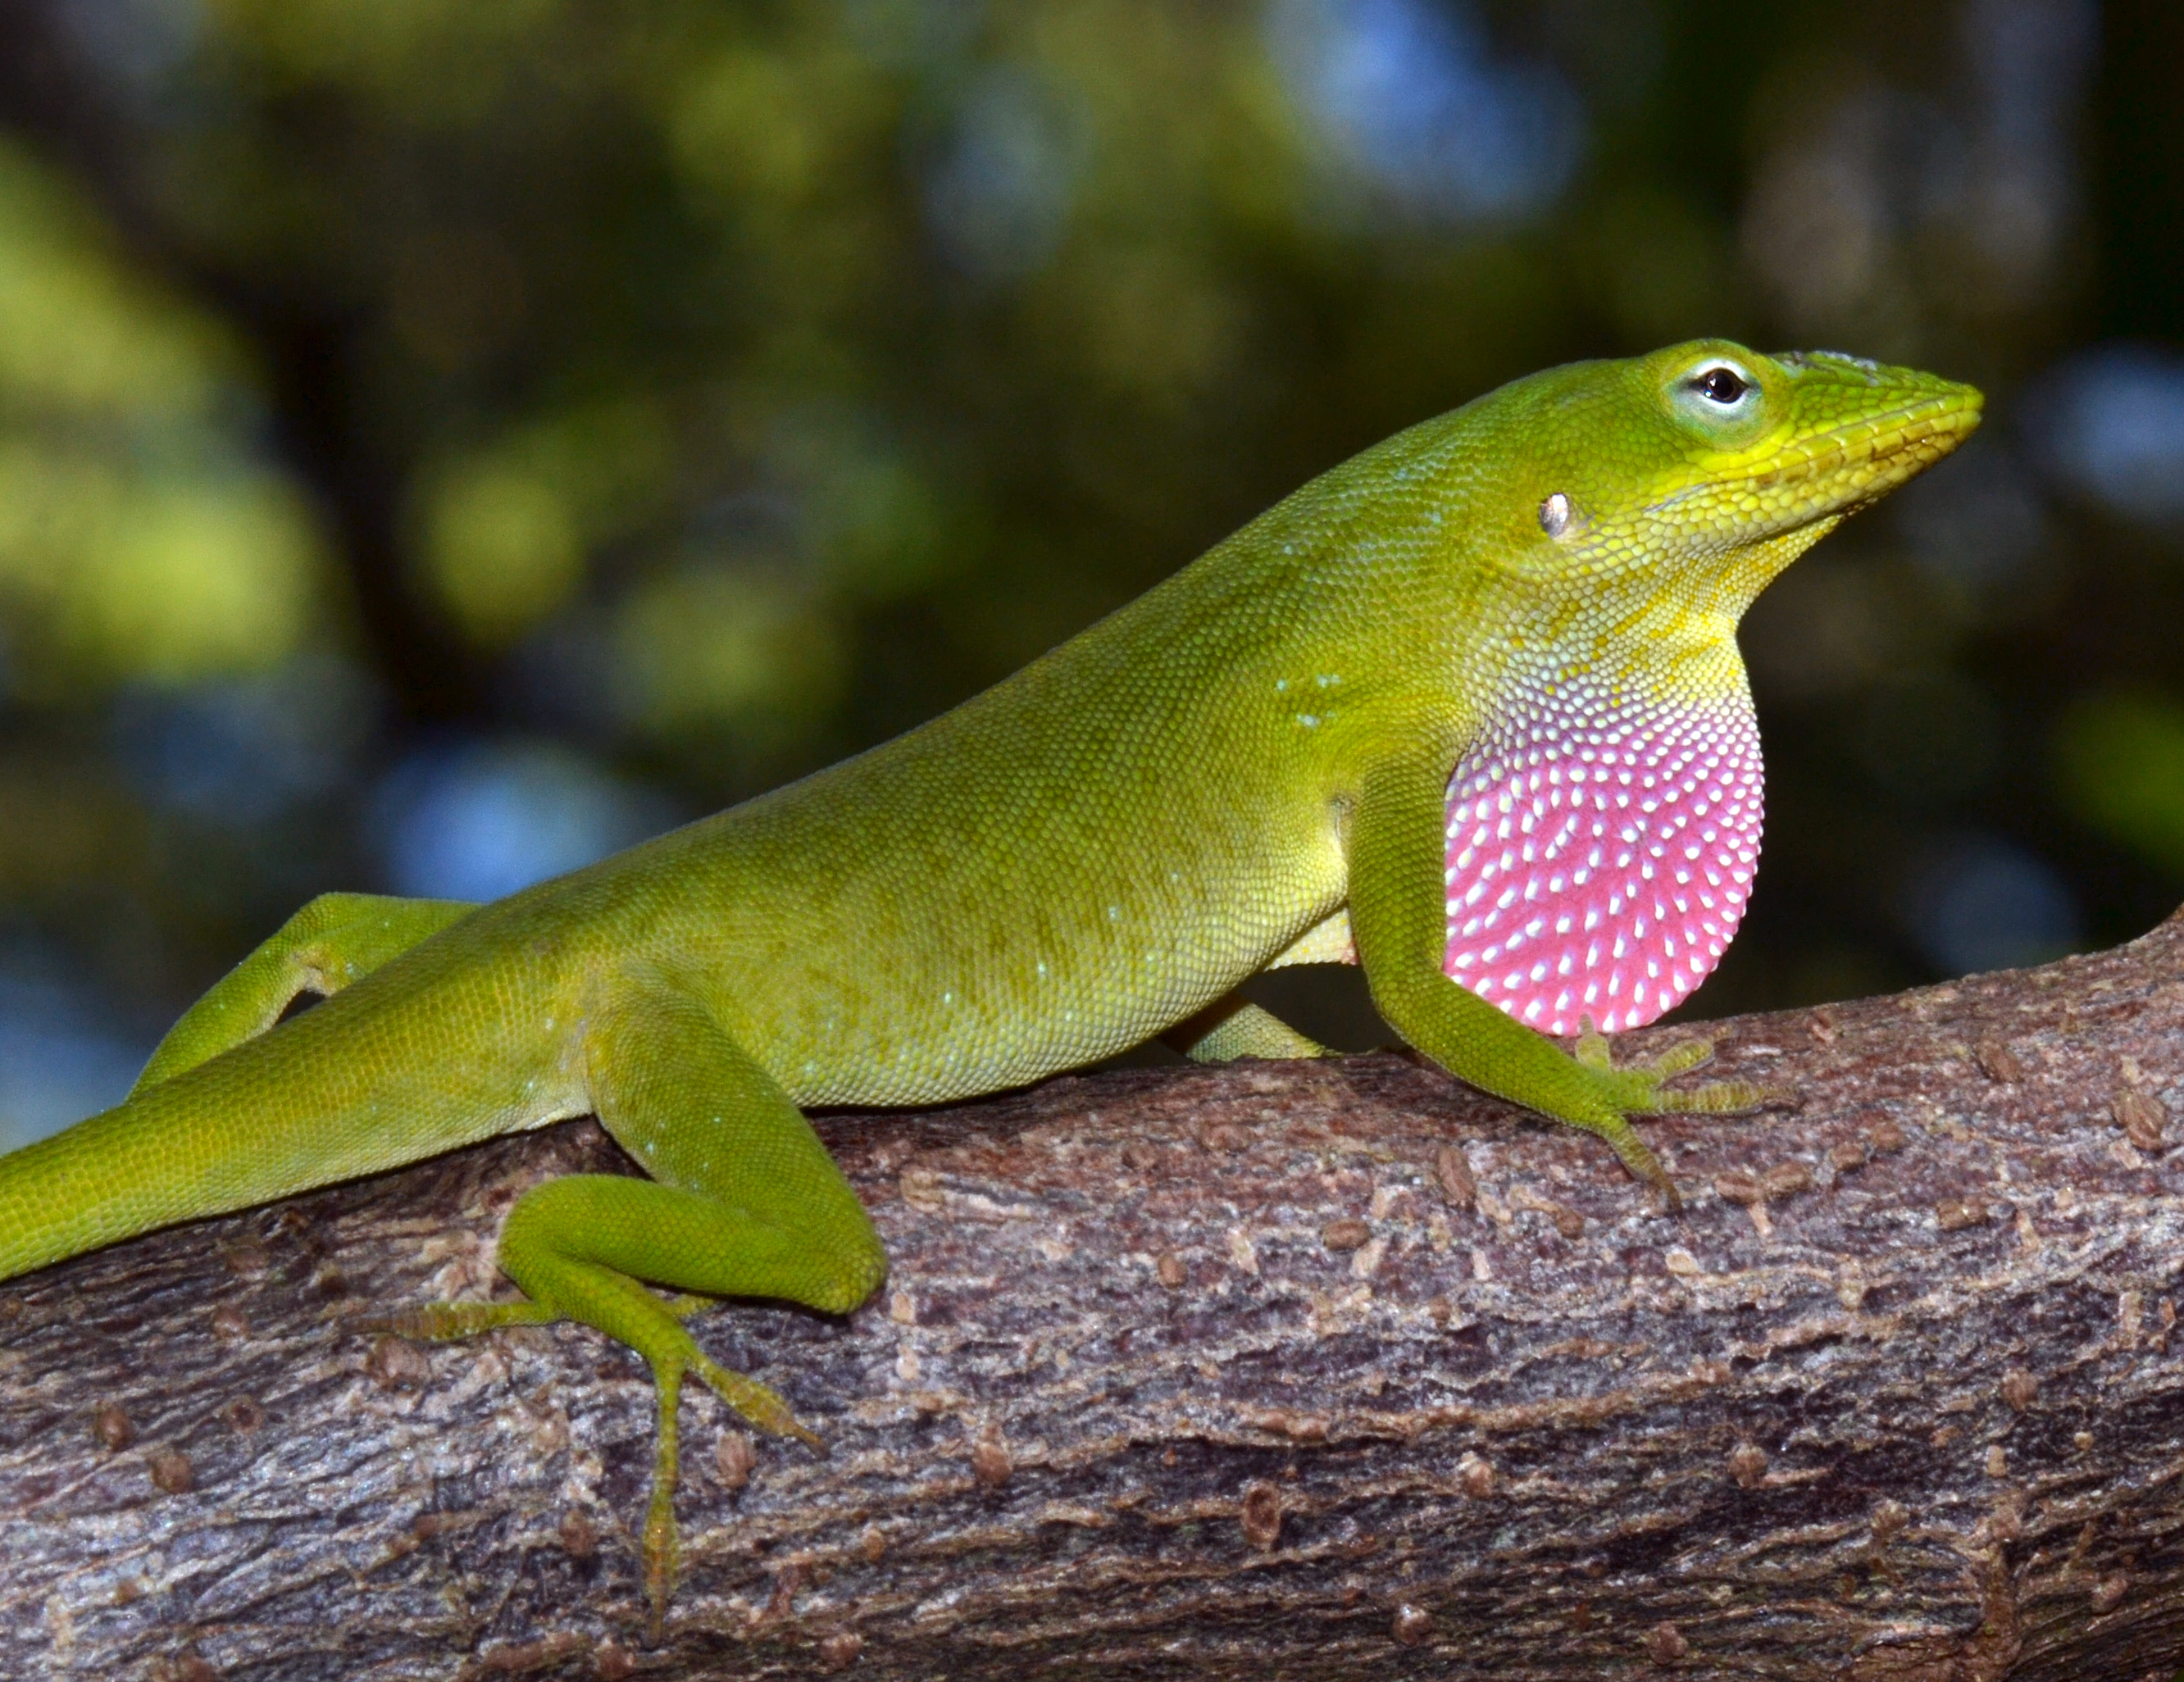
\includegraphics[scale=0.25]{testudines/emydidae/chrysemys/1}
\includegraphics[scale=0.4]{testudines/emydidae/chrysemys/2}
\end{center}